\chapter{Materials \& Methods}
\label{method}

%This section should include a recipe of what you did (explain what you have done so if someone wants to reproduce the experiment, they can).  A flow chart is typically helpful.  Also, make sure to define all software that you used including version numbers and OS.  Should also include a description of statistical methods used (if any).

%Introducing preamble including the schematic of the methodology

%%%%%%%%%%%%%%%%%%%%%%%%%%%%%%%%%%%%%%%%%%%%%%%%%%%%%%%%%%%%%%
\section{Preliminary Study}%%%%%%%%%%%%%%%%%%%%%%%%%%%%%%%%%%%%%%%%%%%%%%
%%%%%%%%%%%%%%%%%%%%%%%%%%%%%%%%%%%%%%%%%%%%%%%%%%%%%%%%%%%%%%
\label{method:prelim study}
%JP comment: explain what 'preliminary study' is
% Ask for references of HPLC and LLE
The transcriptomic data used as the basis of this dissertation originates from the doctoral study of Dr Vassallo Gatt  \citep{Gatt2016}. Three samples of the \ac{ATRA}-resistant HL-60 cell line were incubated and treated with a phenol mixture for varying lengths of time (1, 6, and 12 hours), while a fourth sample served as the negative control, using the growth medium RPMI 1640 as the 'treatment'. This section is a summary of the laboratory procedure utilised by Dr Vassallo Gatt, and is intended to give context to the data.

%%%%%%%%%%%%%%%%%%%%%%%%%%%%%%%%%%%%%%%%%%%%%%%%%%%%%%%%%%%%%%
\subsection{Phenolic extraction}%%%%%%%%%%%%%%%%%%%%%%%%%%%%%%%%%%%%%%%%%%%
%%%%%%%%%%%%%%%%%%%%%%%%%%%%%%%%%%%%%%%%%%%%%%%%%%%%%%%%%%%%%%
Phenolic compounds were isolated from Maltese extra-virgin olive oil by \ac{LLE}, followed by separation of fractions using preparative-scale \ac{HPLC}. \ac{LLE} transferred the water-soluble compounds (including phenols) from their organic solvent to an aqueous one. The heavier aqueous solution was extracted using a separating funnel while the raffinate was discarded. \ac{HPLC} was used to separate the components of the remaining solution based on their differing chemical interactions with an adsorbent column. As the solution was pumped through the column, phenols flowed at a different rate from the other compounds, leading to the isolation of the phenolic fraction. This is likely a mixture of phenols which requires further analysis to determine its chemical composition and to identify the active compound(s).

%%%%%%%%%%%%%%%%%%%%%%%%%%%%%%%%%%%%%%%%%%%%%%%%%%%%%%%%%%%%%%
\subsection{Cell Culturing and RNA extraction}%%%%%%%%%%%%%%%%%%%%%%%%%%%%%%%%%%%
%%%%%%%%%%%%%%%%%%%%%%%%%%%%%%%%%%%%%%%%%%%%%%%%%%%%%%%%%%%%%%
\ac{ATRA}-resistant HL-60 cells were mixed with the phenolic fraction and the mixture was used to seed three wells out of a 6-well plate. The control was seeded similarly, but with growth medium instead of the phenols, which should theoretically not effect their growth. Samples were incubated for their stipulated time period, after which the treated cells began showing characteristic morphological signs of differentiation such as the presence of lobed nuclei, vacuoles, and a decreased nucleus:cytoplasm ratio.

The samples were frozen, then thawed on ice and subjected to RNA extraction according to the RNeasy® Mini kit \citep{RNeasy}, which makes use of the acid guanidinium thiocyanate-phenol-chloroform (AGPC) extraction technique \citep{chomczynski1987single}. This involved the separation of the mixture into two partitions: an organic phase containing DNA and protein, and an aqueous phase containing the RNA, induced by the addition of chloroform. The aqueous phase was separated into a separate microcentrifuge tube to which ethanol was added for precipitation of nucleic acids. The mixture was subjected to multiple cycles of spin column-based nucleic acid purification. Between centrifugation cycles the flow-though was discarded and lysis buffer was added to remove silica-bound proteins, carbohydrates, fatty acids and any traces of salts \citep{matson2009microarray}. A final centrifugation was performed to elute the RNA in RNase-free water.

%%%%%%%%%%%%%%%%%%%%%%%%%%%%%%%%%%%%%%%%%%%%%%%%%%%%%%%%%%%%%%
\subsection{Determination of RNA Quality and Sequencing}%%%%%%%%%%%%%%%%%%%%%%%%%%%
%%%%%%%%%%%%%%%%%%%%%%%%%%%%%%%%%%%%%%%%%%%%%%%%%%%%%%%%%%%%%%
The RNA was analysed using a NanoDrop 2000 UV-Vis Spectrophotometer (Thermo Scientific) which confirmed that the concentrations and A260/280 values were of acceptable quality. The total RNA extracted was then shipped to the \ac{EMBL} in Heidelberg, Germany where the RNA integrity was analysed by gel analysis and then sequenced using an Illumina HiSeq 2000 Sequencing System. The steps followed were typical of the Illumina Stranded mRNA-seq workflow \citep{HiSeq2000}, consisting of poly-A enrichment, RNA fragmentation, cDNA synthesis, ligation of TruSeq adapters, cluster generation, sequencing by synthesis, sequence identification, demultiplexing of the data and the assignment of Phred (Q) scores to each base call \citep{zhong2011high, wang2011low, pease2012rapid}.

The transcriptomic data was received in the form of four FASTQ \citep{cock2010sanger} files, one per experimental time point. They were composed of 51 base-pairs (bp) single-ended reads, with 30x coverage, and were Sanger/Illumina 1.9 encoded, which uses the ASCII character corresponding to the Phred score, and adds '33' to it \citep{ewing1998base}. These served as the starting point for the bulk RNAseq pipeline.

%%%%%%%%%%%%%%%%%%%%%%%%%%%%%%%%%%%%%%%%%%%%%%%%%%%%%%%%%%%%%%
\section{RNA-seq Pipeline}%%%%%%%%%%%%%%%%%%%%%%%%%%%%%%%%%%%%%%%%%%%%%%
%%%%%%%%%%%%%%%%%%%%%%%%%%%%%%%%%%%%%%%%%%%%%%%%%%%%%%%%%%%%%%
RNA-seq analysis is performed in a number of steps, each requiring one or more different tools. The data 'flows' through these tools, which are constituents of the pipeline. Choosing the correct tools is a non-trivial task, and the process is explained further in Section \ref{???}. Each step and tool used in this pipeline is covered in detail in Section \ref{RNA-seq: in silico}. The pipeline for this analysis is represented as the flowchart in \autoref{fig:Dissertation_pipeline}.

Data was stored and processed until the Quantification stage on a high performance computer, managed by the University of Malta with the following specifications: 56-core Intel(R) Xeon(R) CPU E5-2660 v4 @ 2.00GHz with 128GB RAM, running the Ubuntu v18.04.5 operating system. Read count data was then transferred to a VirtualBox v6.1.32 \citep{virtualbox} virtual environment running Ubuntu v20.04.4, with the following partitioned resources: Intel(R) Core(TM) i5-7200U CPU @ 2.50GHz with 4GB RAM.
% NOTE: FIGURE IS NOT ACCURATE. PLEASE REVISIT
\begin{figure}[!ht]
    \centering
    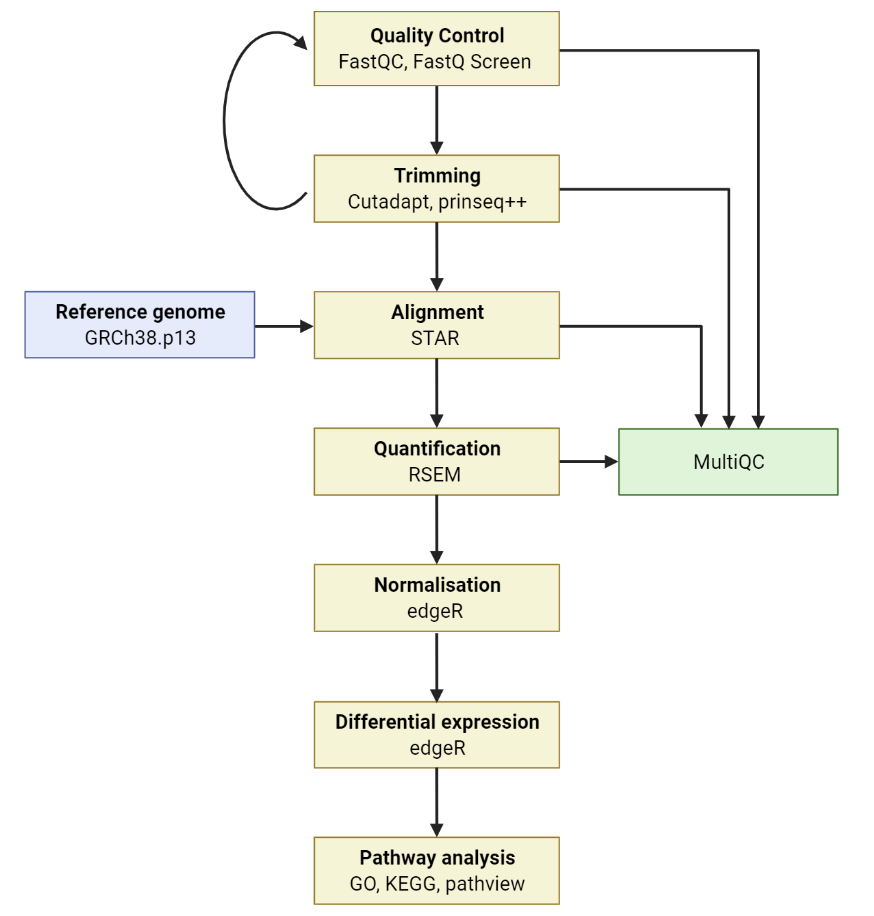
\includegraphics[width=1\textwidth]{Dissertation_pipeline}
    \caption[General overview of the RNA-seq pipeline.]{General overview of the RNA-seq pipeline. Created with \href{https://biorender.com/}{BioRender.com}.} 
    \label{fig:Dissertation_pipeline}
\end{figure}

\clearpage
%%%%%%%%%%%%%%%%%%%%%%%%%%%%%%%%%%%%%%%%%%%%%%%%%%%%%%%%%%%%%%
\subsection{Quality Control}%%%%%%%%%%%%%%%%%%%%%%%%%%%%%%%%%%%%%%%%%%%%%
%%%%%%%%%%%%%%%%%%%%%%%%%%%%%%%%%%%%%%%%%%%%%%%%%%%%%%%%%%%%%%
% Maybe list used arguments and their use like evas documentation??

The first step of any sequencing pipeline should be the assessment of the quality of the raw data files. Sequencing information of poor quality is identified if present, and if necessary, truncated to mitigate inaccuracies in the downstream pipeline. To assess the quality of the FASTQ files, they were ported to FastQC v0.11.9 \citep{andrews2010fastqc} using eight threads (\autoref{lst:FastQC}). This extracted information on the sequences, including Phred scores, GC content, N content, sequence length distribution, sequence duplication levels, overrepresented sequences and adapter sequences. FastQC rates each of these modules using a green check-mark signifying that it 'passed' QC, a yellow exclamation mark 'warning', or a red cross 'failed'. 

Two modules failed consistently throughout the four samples received: 'Sequence Duplication Levels' and 'Per base sequence content'. This is normal and expected for RNA data, and is explained in further detail in \autoref{Assessing the Quality of the Raw FASTQ files}. Traces (<0.5\%) of TruSeq adapters were detected in the FASTQ files, which is corroborated by the sequencer's manual \citep{HiSeq2000} stating that it makes use of the 'TruSeq family of reagents'. 

\begin{lstlisting}[language=bash, caption=FastQC command, label={lst:FastQC}]
# FastQC accepts multiple input files, so we can use wildcards
fastqc \
 -t 8 \
 -o ./raw_FastQC_out \
*.fq 
\end{lstlisting}

Next, Fastq Screen v0.14.0 \citep{wingett2018fastq} was used to check for RNA contaminants from other common sources, by comparing the reads against a set of sequence databases (\autoref{lst:FastqScreen}). Perl, an aligner (Bowtie \citep{bowtie}, Bowtie2 \citep{bowtie2} or BWA \citep{bwa}) and a Linux-based operating system are required. Bowtie2 was used to align the sample reads to the reads in the contaminant database.

\begin{lstlisting}[language=bash, caption=FastqScreen command, label={lst:FastqScreen}]
# FastQScreen also accepts multiple file inputs
fastq_screen \
--aligner bowtie2 \
--conf ./fastq_screen.conf \
 *.fq 
\end{lstlisting}


%%%%%%%%%%%%%%%%%%%%%%%%%%%%%%%%%%%%%%%%%%%%%%%%%%%%%%%%%%%%%%
\subsection{Preprocessing}%%%%%%%%%%%%%%%%%%%%%%%%%%%%%%%%%%%%%%%%%%%%%%
%%%%%%%%%%%%%%%%%%%%%%%%%%%%%%%%%%%%%%%%%%%%%%%%%%%%%%%%%%%%%%
Poor quality reads lead to poor downstream sequence analysis. Thus, it is common practice in RNA-seq to trim the undesired regions. Cutadapt \citep{martin2011cutadapt} was used to trim the previously detected TruSeq adapter sequences and short reads, using a threshold of <45 bp. Between 1.3 and 1.6\% of the base-pairs were trimmed across the four samples. Cutadapt was accessed through the wrapper script Trim Galore! v0.6.7 \citep{trimgalore} which instantly redirects the trimmed data back to FastQC to assess the improvement in quality, if any.

\begin{lstlisting}[caption=Trim Galore! trimming]
trim_galore \
--phred33 \
--fastqc \
-a "GATCGGAAGAGCACACGTCTGAACTCCAGTCAC" \
--length 45 \
-o trim_galore_output \
--fastqc_args "-o trimmed_FastQC_out -t 8" \
--cores 4 \
*.fq 
\end{lstlisting}

The trimmed files were further filtered using Prinseq++ \citep{prinseq++} which removed ambiguous reads containing >7 N's and sequences with a DUST score\footnote{A value between 0 and 1 generated by the DUST algorithm which is a measure of sequence complexity. Here, its purpose is to mask low-complexity regions.} of <0.1.

\begin{lstlisting}[caption=Prinseq++ filtering]
samples=(control, 1hour, 6hour, 12hour)
mkdir prinseq_out

for sample in ${samples[@]};
do
        prinseq++ \
        -fastq ./trim_galore_output/${sample}_trimmed.fq \
        -out_name ./prinseq_out/${sample}_filtered.fq \
        -out_bad ./prinseq_out/${sample}_bad.fq \
        -ns_max_n 7 \
        -lc_dust=0.1 > ./prinseq_out/control_prinseq_report.txt
done
\end{lstlisting}

\subsection{Read alignment and Quantification}
The trimmed and filtered FASTQ files were aligned to the GRCh38.p13 reference genome \citep{ref} using the \ac{STAR} 2.7.9a aligner \citep{Dobin2013}. \ac{STAR} was called through RSEM v1.3.3 \citep{li2011rsem}, which after alignment estimates gene and isoform expression levels. RSEM must be accessed through a 64 bit Linux or Mac OS command-line, and must have C++, Perl and R installed as dependencies.

Reference transcripts from the reference genome were first generated through the \texttt{rsem-prepare-reference} program, with the help of its respective GTF file (\autoref{lst:RSEM_ref}). 

% .genes.results (one row per gene) which has the headers: gene_id transcript_id(s)        length  effective_length        expected_count  TPM     FPKM
% .isoforms.results (one row per transcript) which has the headers: transcript_id   gene_id length  effective_length        expected_count  TPM     FPKM    IsoPct

\begin{lstlisting}[caption= reference generation, label={lst:RSEM_ref}]
mkdir RSEM
mkdir RSEM/reference
rsem-prepare-reference --gtf mm9.gtf \
                       --star \
                       --star-sjdboverhang 50 \
                       --num-threads 8 \
                       --gtf Homo_sapiens.GRCh38.104.gtf \
                       Homo_sapiens.GRCh38.dna.primary_assembly.fa \
                       ./RSEM/reference/GRCh38
\end{lstlisting}

The \texttt{--star-sjdboverhang} is an argument passed to \ac{STAR} which sets the maximum possible overhang for the reads. It should be equal to the read length minus one. In our case, the read length is 51, thus a value of 50 is used. The final variable is a prefix to the output files. This may be used as the output path for the generated reference files.

To calculate expression values, the \texttt{rsem-calculate-expression} command is used. As before, the final argument is a prefix to the output files, and the argument before that is the path to the reference files created in the previous command. RSEM first uses \ac{STAR} to align the filtered sample reads to the generated reference reads, creating a BAM file sorted by its coordinates. It outputs two quantification files per sample, with differing suffices: one ending in '.genes.results' and another '.isoform.results'. These are both tab-delimited text files with similar headers, with the former dedicating a row for each gene and the latter dedicating a row for each transcript. The isoform-centric file thus contains more data, which are unnecessary for our objectives. Of the columns in the gene-centric file, two will be used in the subsequent step: 'gene\textunderscore id' which holds the Ensembl gene ID, and 'TPM' which holds the normalised read count for the respective gene.

\begin{lstlisting}[caption=RSEM expression command, label={lst:RSEM_exp}]
mkdir RSEM/expression
samples=(control, 1hour, 6hour, 12hour)

for sample in ${samples[@]};
do
        rsem-calculate-expression \
        --num-threads 16 \
        --star \
        --sort-bam-by-coordinate \
        ./prinseq_out/${sample}*good_out.fq \
        ./RSEM/reference/GRCh38 \
        ./RSEM/expression/${sample}
done
\end{lstlisting}

\subsection{Reassessing the Quality}

The produced files from FastQC, FastQScreen, Trim Galore! and RSEM, were funnelled into MultiQC v1.11 \citep{multiqc} which summarises their output in the form of an HTML report. At the time of writing, the latest version of MultiQC did not support Prinseq++ and its log files were inspected manually instead.

\begin{lstlisting}[language=bash, caption=MultiQC command]
multiqc \
-o ./multiqc_out \
./trim_galore_output/*txt \
./fastqc/FastQC_out/. \
./FastQ_Screen_out/raw/. \
./RSEM/expression/.
\end{lstlisting}

\subsection{Normalisation and Differential Gene Expression}
% Find another name for this?

We have chosen edgeR v3.14 \citep{edger} as the package to help identify differentially expressed genes, which supports datasets that lack replicates such as our own. The instructions on the vignette\footnote{\url{https://www.bioconductor.org/packages/release/bioc/vignettes/edgeR/inst/doc/edgeRUsersGuide.pdf}} were followed, and are summarised as follows. 

The four gene read count files generated through RSEM were imported into the R script v3.6.3 \citep{R} and had their gene IDs (1st column) and expected read counts (5th column) compiled into a single \texttt{DGEList} object which consists of multiple data-frames. 

\begin{lstlisting}[language=R, caption=Importing count files to R]
files <- list("1hour.genes.results", "12hour.genes.results", 
"6hour.genes.results", "control.genes.results")
path <- "/path/to/files/"
labels = c('1hr', '12hr', '6hr', '0hr')
group <- factor(labels)
y <- readDGE(files, path=path, columns=c(1,5), group=group, labels=labels)
\end{lstlisting}

\subsubsection{Filtering Low Count Genes}

Genes with low counts (<10) are generally considered as noise, as they are not expressed at any biologically meaningful level and filtering them would reduce the amount of statistical tests required in the downstream analysis \citep{law2016rna}. EdgeR provides the function \texttt{filterByExpr} which serves this purpose.

\begin{lstlisting}[language=R, caption=Filtering low count genes]
library(edgeR)
keep <- filterByExpr(y, group=group)
table(keep)  # How many genes were removed and how many remain
y <- y[keep,keep.lib.sizes=FALSE]
\end{lstlisting}

\subsubsection{Gene Annotation}

The remaining genes were annotated using the AnnotationDbi library v3.14 \citep{annotationdbi} which is dependent on the org.Hs.eg.db v3.10.0 \citep{org.Hs.eg.db} human annotation database. These were used to add the Entrez ID annotation to the \texttt{DGEList} object, which will be used for pathway analysis further downstream. AnnotationDbi provides other useful annotation options, but were excluded as  combination of annotations was causing a one to many mapping error. This step was later repeated (after pathway analysis) to add gene symbol annotations. This proved useful for later research into their biology, since most papers refer to the gene by its gene symbol.

\begin{lstlisting}[language=R, caption=Annotation step]
library(org.Hs.eg.db)
library(AnnotationDbi) 

# This step was repeated at a later stage with "SYMBOL" as the
# column argument, which adds the gene symbol.
Symbol <- mapIds(org.Hs.eg.db, keys=rownames(y), keytype="ENSEMBL",
                 column="ENTREZID")

y$genes <- data.frame(Symbol=Symbol)
head(y$genes)
\end{lstlisting}

\subsubsection{Normalisation}

The read counts are then normalised by the \texttt{calcNormFactors} function which uses the \ac{TMM} method. This is recommended by the edgeR vignette and is explained in detail in \cite{robinson2010scaling}. The aim of normalisation is to mitigate any technical bias on the data.
% Maybe write more here

\begin{lstlisting}[language=R, caption=TMM normalisation]
y <- calcNormFactors(y)
design <- model.matrix(~group)
\end{lstlisting}

EdgeR has multiple methods to determine which genes are differentially expressed, but the classic \texttt{exactTest} was deemed as most appropriate. This is a pairwise test which compares the means between two groups of counts with a negative-binomial distribution. The calculation of the dispersion of our data is required prior to its use, however this is not mathematically possible due to our lack of replicates. In such cases the edgeR vignette suggests that estimating the dispersion based on the experimental conditions is more scientifically sound than assuming no variation. It should be emphasised that this technique is inaccurate, but was deemed as the best possible option for statistical analysis without replicates (further detail in Section \ref{Adapting Differential Gene Expression Analysis to a Lack of Replicates}).

The \ac{BCV} is equal to the square root of the dispersion, and the vignette suggests a few estimates for the \ac{BCV}, such as '0.1 for data on genetically identical model organisms'. While this is human data, not a model organism, the data originate from the same genetically identical cell line, and this value was deemed appropriate. Thus the dispersion used for \texttt{exactTest} is equal to the BCV\textsuperscript{2}, or 0.01. 
The test was performed a total of three times, where each treated sample was compared with the control. This returns a \texttt{DGEExact} object for each comparison, containing the $log_{2}$ fold change (logFC), $log_{2}$ Counts Per Million (logCPM), p-values and annotations for each gene. 

\begin{lstlisting}[language=R, caption=Exact test function]
bcv <- 0.1
et_12 <- exactTest(y, pair=c(1, 2), dispersion=bcv^2)
et_1 <- exactTest(y, pair=c(1, 3), dispersion=bcv^2)
et_6 <- exactTest(y, pair=c(1, 4), dispersion=bcv^2)
\end{lstlisting}

% EdgeR has three ways of judging differential expression but exactTest was deemed as the best fit

\subsubsection{Adjusting p-values and Cut-offs}

Multiple testing is an inherent risk of RNA-seq due to its vast amounts of comparisons and adjusting p-values is a common technique implemented into the RNAseq pipeline to help compensate for this.  The \ac{FDR} with the Benjamini-Hochberg controlling procedure was the chosen p-value adjustment method. This produced value is the proportion of false positives one might expect to get from a test. Each of the \texttt{DGEExact} objects was transformed in this way using the \texttt{topTags} function. Differential expression was sorted by the \ac{FDR} and any genes with an \ac{FDR} < 0.05 were filtered out, which means that we are willing to accept that 5\% of all \ac{DEG} will be false positives. Filtering on the logFC was then performed manually, using a threshold of 1.5.  

%Summary of  https://www.science.smith.edu/cmbs/wp-content/uploads/sites/36/2015/09/P-and-q-values-in-RNA-Seq.pdf:
%		FDR makes use of Q-values which usually result in a smaller number of false positives, although this is not always the case:
%		An FDR-adjusted p-value (aka a q-value) of 0.05 implies that we are willing to accept that 5% of the tests found to be statistically significant (e.g. by p-value) will be false positives

%'Many traditional techniques such as the Bonferroni correction are too conservative in the sense that while they reduce the number of false positives, they also reduce the number of true discoveries.': https://www.nonlinear.com/support/progenesis/comet/faq/v2.0/pq-values.aspx

\begin{lstlisting}[language=R, caption=Adjusting p-values and filtering data based on the logFC and FDR]
FDR_thresh <- 0.05  # removes rows with FDR less than this
et_1_toptags <- topTags(et_1, n=nrow(et_1$table), adjust.method="BH", 
sort.by="PValue", p.value=FDR_thresh)$table
et_12_toptags <- topTags(et_12, n=nrow(et_12$table), adjust.method="BH", 
sort.by="PValue", p.value=FDR_thresh)$table
et_6_toptags <- topTags(et_6, n=nrow(et_6$table), adjust.method="BH", 
sort.by="PValue", p.value=FDR_thresh)$table

FC_thresh <- 1.5  # removes rows with a logFC less than this
et_1_toptags <- et_1_toptags[abs(et_1_toptags$logFC) > FC_thresh, ]
et_12_toptags <- et_12_toptags[abs(et_12_toptags$logFC) > FC_thresh, ]
et_6_toptags <- et_6_toptags[abs(et_6_toptags$logFC) > FC_thresh, ]
\end{lstlisting}

\subsection{Functional analysis}
?

% The main components of an DGEList object are a matrix counts containing the integer counts,
% a data.frame samples containing information about the samples or libraries, and a optional
% data.frame genes containing annotation for the genes or genomic features


%EdgeR manual:
%A commonly used approach is to conduct DE tests, apply a fold-change cut-off and then rank all the genes above that fold-change threshold by p-value. In some other cases genes are first chosen according to a p-value cut-off and then sorted by their fold-changes.

%\subsubsection{Gene Set Enrichment Analysis and Pathway Analysis}
%\ac{GO}
%\ac{KEGG}
% https://www.biostars.org/p/462980/
% pathways
% library(pathview)
% HOUSEKEEPING GENES for sanity checks 
%https://www.genomics-online.com/resources/16/5049/housekeeping-genes/

\section{Summary}
Empty for now.
